\documentclass[11pt,a4paper]{article}
\usepackage[utf8]{inputenc}
\usepackage[T1]{fontenc}
\usepackage[brazil]{babel}
\usepackage{lmodern}
\usepackage{microtype}
\usepackage{geometry}
\usepackage{amsmath,amssymb}
\usepackage{booktabs}
\usepackage{longtable}
\usepackage{array}
\usepackage{graphicx}
\usepackage{float}
\usepackage{caption}
\usepackage{listings}
\usepackage{xcolor}
\usepackage{hyperref}
\geometry{top=2.5cm,bottom=2.5cm,left=3cm,right=2cm}
\hypersetup{colorlinks=true,linkcolor=black,urlcolor=black,citecolor=black,pdftitle={Trabalho Prático 1 - Cálculo Numérico}}
\DeclareUnicodeCharacter{00B7}{\ensuremath{\cdot}}
\renewcommand{\arraystretch}{1.18}
\captionsetup{font=small,labelfont=bf}
\lstset{basicstyle=\ttfamily\scriptsize,breaklines=true,frame=single,columns=fullflexible,showstringspaces=false}

\begin{document}

\begin{titlepage}
\centering
\vspace*{1.0cm}

\includegraphics[width=0.28\textwidth]{figures/brasao_ufsc_oficial.png}\\[1.0cm]
{\large \textsc{Universidade Federal de Santa Catarina}}\\[0.2cm]
{\large Departamento de Automação e Sistemas}\\[2.6cm]
{\Large DAS-5103 -- Cálculo Numérico para Controle e Automação}\\[1.4cm]
{\LARGE\bfseries Trabalho Prático 1}\\[2.8cm]
{\large João Victor Barbosa Teixeira Bouças}\\[0.2cm]
{\large Matrícula 25103276}\\[3.0cm]
{\large Florianópolis}\\[0.2cm]
{\large 2026}
\end{titlepage}

\pagenumbering{arabic}

\section{Introdução}

Este relatório trata de três classes de problemas numéricos: a determinação de uma raiz escalar, a solução de um sistema linear e a solução de um sistema não linear. Em cada caso foram implementados em Python os algoritmos especificados no enunciado, sem recorrer a rotinas prontas de busca de raízes ou de solução de sistemas como procedimento principal.

Além dos valores finais, foram examinados os resíduos, o número de iterações e as trajetórias dos iterandos. Os critérios de parada não foram escolhidos livremente: para a Questão 1, adotou-se $|f(\theta_k)|<10^{-5}$; para a Questão 3, $\lVert F(x_k)\rVert_2\leq 10^{-5}$; em ambos os casos o limite foi de 100 iterações. A discussão dos métodos segue as definições e os cuidados de convergência apresentados nas notas da disciplina \cite{notas}.

\section{Questão 1 -- Equação não linear}

\subsection{Formulação e métodos}

Para o alcance horizontal do foguete, foi resolvida a equação
\begin{equation}
f(\theta)=\frac{100^2}{9,8}\left[\sin(\theta)+0,5\sin(2\theta)\right]-1000=0,
\end{equation}
no domínio de interesse $0\leq\theta\leq\pi/2$. As avaliações iniciais foram $f(0,5)=-81,468335706$ e $f(1,5)=89,852031259$. Logo, o intervalo usado nos métodos de quebra contém mudança de sinal e está integralmente no domínio estabelecido.

Foram aplicados bisseção, falsa posição, Newton e secante com os pontos iniciais prescritos. Na bisseção, o intervalo com sinais opostos foi preservado e dividido ao meio a cada passo. A falsa posição preservou a mesma propriedade, mas escolheu a interseção da secante dos extremos com o eixo horizontal. Newton usou a derivada analítica
\begin{equation}
f'(\theta)=\frac{100^2}{9,8}\left[\cos(\theta)+\cos(2\theta)\right],
\end{equation}
e a secante substituiu essa derivada por uma inclinação calculada com os dois iterandos anteriores.

\subsection{Resultados e validação}

As Figuras \ref{fig:q1theta} e \ref{fig:q1residuo} registram todos os iterandos efetivamente gerados até o critério de parada. A escala logarítmica na Figura \ref{fig:q1residuo} permite distinguir a velocidade com que os resíduos se aproximam da tolerância.

\begin{figure}[H]
\centering
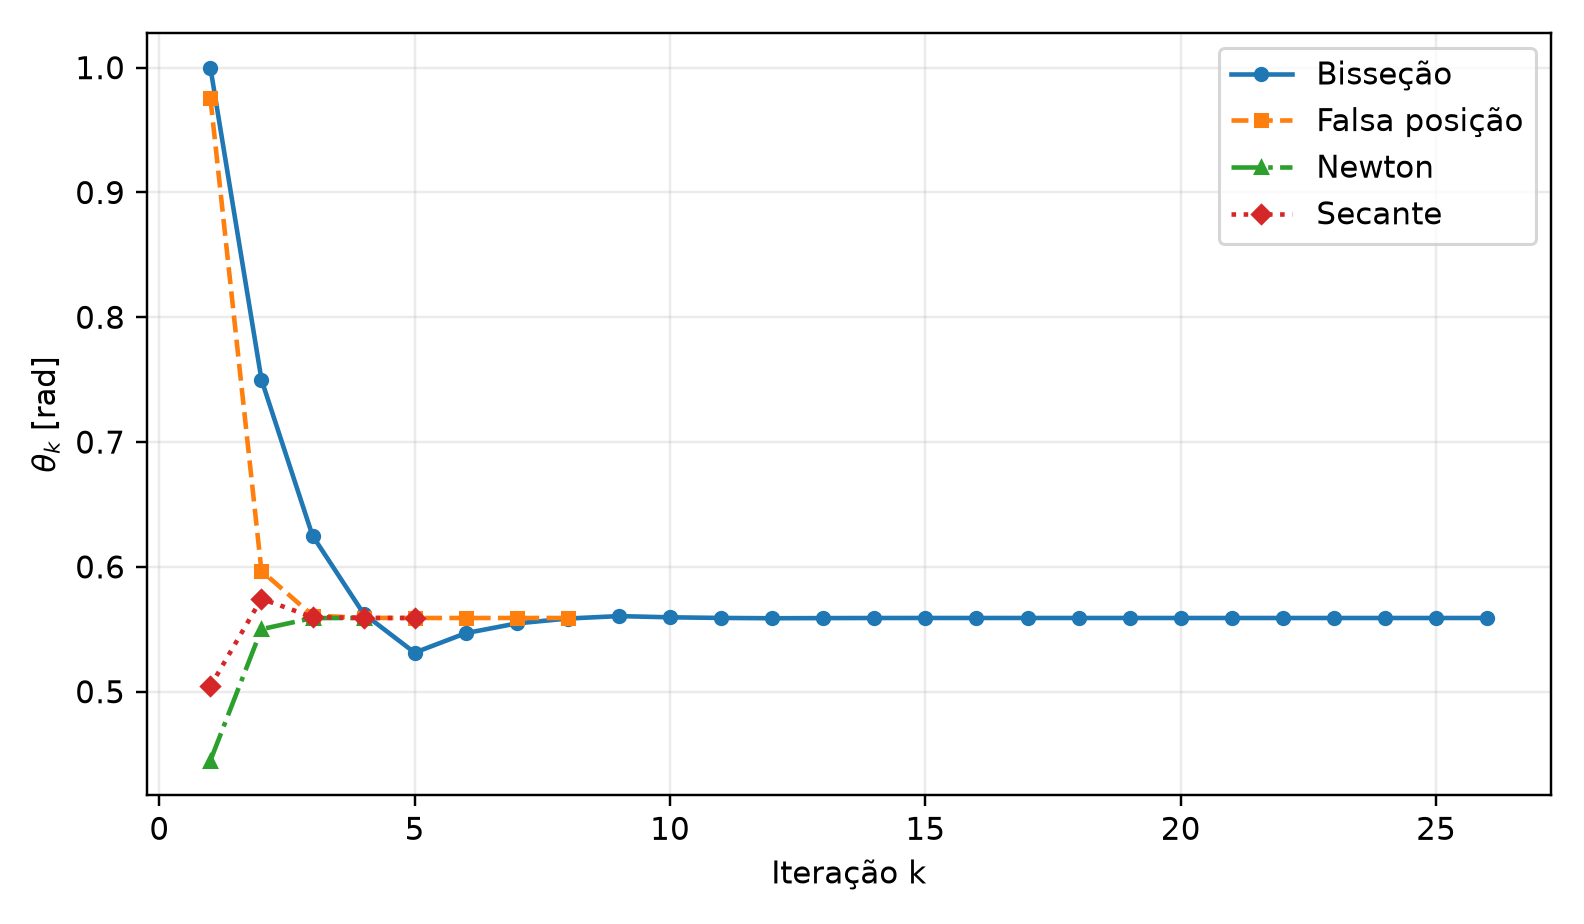
\includegraphics[width=0.83\textwidth]{figures/q1_theta_iteracoes.png}
\caption{Trajetória de $\theta_k$ para os quatro métodos da Questão 1.}
\label{fig:q1theta}
\end{figure}

\begin{figure}[H]
\centering
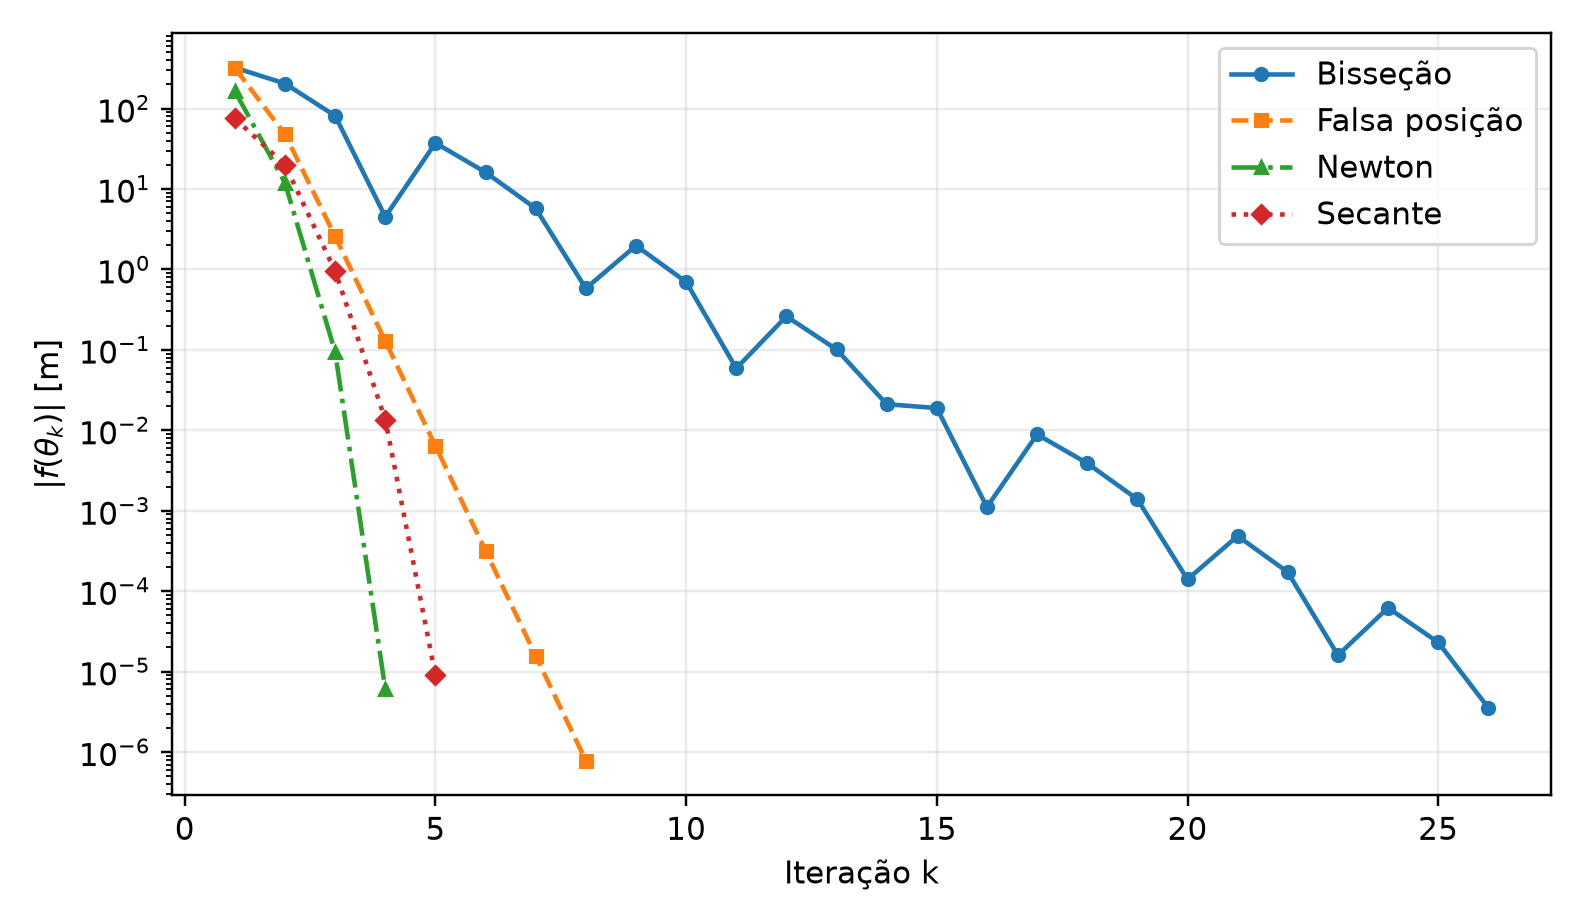
\includegraphics[width=0.83\textwidth]{figures/q1_residuo_iteracoes.png}
\caption{Módulo do resíduo por iteração na Questão 1.}
\label{fig:q1residuo}
\end{figure}

\begin{table}[H]
\centering
\caption{Comparação final dos métodos para a Questão 1.}
\label{tab:q1}
\begin{tabular}{lrrrrl}
\toprule
Método & $\theta$ [rad] & $\theta$ [graus] & Iterações & $|f(\theta)|$ & Situação \\
\midrule
Bisseção & 0,559037104 & 32,030466665 & 26 & $3,549\times10^{-6}$ & Convergiu \\
Falsa posição & 0,559037102 & 32,030466544 & 8 & $7,821\times10^{-7}$ & Convergiu \\
Newton & 0,559037097 & 32,030466245 & 4 & $6,058\times10^{-6}$ & Convergiu \\
Secante & 0,559037108 & 32,030466902 & 5 & $8,971\times10^{-6}$ & Convergiu \\
\bottomrule
\end{tabular}
\end{table}

As quatro aproximações pertencem ao domínio e concordam até as casas apresentadas. A substituição direta de cada uma em $f$ produz os resíduos da Tabela \ref{tab:q1}; portanto, todas satisfazem o critério determinado no enunciado. A bisseção foi a mais lenta, como se espera da redução controlada do intervalo. Em contrapartida, ela conservou a garantia associada à mudança de sinal em todas as 26 iterações.

Na falsa posição, não ocorreu o problema de uma extremidade ficar praticamente fixa: o resíduo atingiu a tolerância em oito passos. O método de Newton foi o mais rápido neste caso, com quatro passos a partir de $\theta_0=0,8$; a derivada não se aproximou de zero na trajetória registrada, de modo que o risco de um passo excessivo associado a uma derivada pequena não se materializou. A secante convergiu em cinco passos e não apresentou denominador próximo de zero. Esses dois últimos métodos foram rápidos porque os pontos prescritos estavam em uma região favorável da raiz, mas não possuem a proteção global fornecida pelo intervalo com mudança de sinal.

\subsection{Conclusão da questão}

O ângulo de lançamento obtido é aproximadamente $0,5590371$ rad, ou $32,03047^\circ$. A comparação dos resíduos mostra convergência de todos os métodos; a diferença relevante está no custo iterativo: 26 passos para a bisseção, 8 para a falsa posição, 4 para Newton e 5 para a secante. Neste problema, Newton atingiu a tolerância com menos iterações, enquanto a bisseção ofereceu a trajetória mais previsível por manter o intervalo válido.

\section{Questão 2 -- Sistema de equações lineares}

\subsection{Sistema e leitura do grafo}

O sistema fornecido no enunciado foi escrito na forma $Ax=b$ na ordem $(x_1,\ldots,x_7)^T$. A imagem da malha aérea contém arcos curvos que se cruzam e rótulos próximos de outros trechos. Por esse motivo, a leitura adotada não foi baseada na geometria ou no cruzamento visual das linhas. Cada arco foi identificado pelo rótulo $x_i$, e seu sentido foi fixado pela tabela de resultados e pelas equações do enunciado, que são a especificação formal do problema. O Quadro \ref{tab:leitura-grafo} documenta essa transcrição.

\begin{table}[H]
\centering
\caption{Transcrição orientada usada para interpretar a figura da Questão 2.}
\label{tab:leitura-grafo}
\begin{tabular}{cll}
\toprule
Variável & Rota lida & Critério de leitura \\
\midrule
$x_1$ & IGU $\rightarrow$ GRU & Rótulo e tabela do enunciado \\
$x_2$ & GRU $\rightarrow$ Outros & Rótulo e tabela do enunciado \\
$x_3$ & Outros $\rightarrow$ GIG & Rótulo e tabela do enunciado \\
$x_4$ & GIG $\rightarrow$ POA & Rótulo e tabela do enunciado \\
$x_5$ & POA $\rightarrow$ CGH & Rótulo e tabela do enunciado \\
$x_6$ & SDU $\rightarrow$ CGH & Rótulo e tabela do enunciado \\
$x_7$ & CGH $\rightarrow$ IGU & Rótulo e tabela do enunciado \\
\bottomrule
\end{tabular}
\end{table}

Assim, os cruzamentos no desenho são apenas sobreposições de arcos no plano e não conexões entre aeroportos. A equação $-x_1+2x_7=0$ foi tratada como a relação adicional informada pelo enunciado, isto é, $x_1=2x_7$; ela não foi deduzida de uma leitura espacial do desenho.

\subsection{Eliminação de Gauss com pivotamento}

Foi implementada eliminação de Gauss com pivotamento parcial, seguida de retrosubstituição. Em cada coluna, seleciona-se a maior entrada em módulo dentre as linhas ainda disponíveis. Isso evita a divisão por pivôs nulos e reduz a exposição a amplificação de arredondamentos quando há pivôs pequenos. Neste sistema, ocorreram empates de módulo iguais a um nas três primeiras colunas; a implementação manteve a primeira linha candidata, portanto não houve troca de linhas. Ainda assim, a seleção do pivô foi executada em cada etapa.

A matriz aumentada inicial é
\[
\left[\begin{array}{rrrrrrr|r}
-1&0&0&0&0&0&2&0\\1&-1&0&0&0&0&0&-130\\0&1&-1&0&0&0&0&102\\0&0&1&-1&0&0&0&22\\0&0&0&1&-1&0&0&-1\\0&0&0&0&0&1&0&29\\0&0&0&0&1&1&-1&38
\end{array}\right].
\]

\paragraph{Etapa 1.} Na coluna 1, escolheu-se a linha 1 como pivô ($a_{11}=-1$). Como $|a_{11}|=|a_{21}|=1$, não há ganho em permutar as duas linhas. O único multiplicador não nulo é $m_{21}=a_{21}/a_{11}=-1$, e a operação é $L_2\leftarrow L_2-(-1)L_1=L_2+L_1$. O resultado é
\[
\left[\begin{array}{rrrrrrr|r}
-1&0&0&0&0&0&2&0\\0&-1&0&0&0&0&2&-130\\0&1&-1&0&0&0&0&102\\0&0&1&-1&0&0&0&22\\0&0&0&1&-1&0&0&-1\\0&0&0&0&0&1&0&29\\0&0&0&0&1&1&-1&38
\end{array}\right].
\]

\paragraph{Etapa 2.} Na coluna 2, a linha 2 permanece pivô ($a_{22}=-1$), em empate de módulo com a linha 3. O multiplicador é $m_{32}=1/(-1)=-1$, portanto $L_3\leftarrow L_3+L_2$. A matriz passa a ser
\[
\left[\begin{array}{rrrrrrr|r}
-1&0&0&0&0&0&2&0\\0&-1&0&0&0&0&2&-130\\0&0&-1&0&0&0&2&-28\\0&0&1&-1&0&0&0&22\\0&0&0&1&-1&0&0&-1\\0&0&0&0&0&1&0&29\\0&0&0&0&1&1&-1&38
\end{array}\right].
\]

\paragraph{Etapa 3.} Na coluna 3, mantém-se a linha 3 como pivô ($a_{33}=-1$), novamente com empate de módulo com a linha 4. O multiplicador é $m_{43}=1/(-1)=-1$, dando $L_4\leftarrow L_4+L_3$. Obtém-se
\[
\left[\begin{array}{rrrrrrr|r}
-1&0&0&0&0&0&2&0\\0&-1&0&0&0&0&2&-130\\0&0&-1&0&0&0&2&-28\\0&0&0&-1&0&0&2&-6\\0&0&0&1&-1&0&0&-1\\0&0&0&0&0&1&0&29\\0&0&0&0&1&1&-1&38
\end{array}\right].
\]

As etapas restantes e a retrosubstituição fornecem
\begin{equation}
x=(4,\ 134,\ 32,\ 10,\ 11,\ 29,\ 2)^T.
\end{equation}

\subsection{Resultados e validação}

\begin{table}[H]
\centering
\caption{Quantidade de voos diários nas rotas desconhecidas.}
\label{tab:q2}
\begin{tabular}{cl r}
\toprule
Variável & Voo & Voos por dia \\
\midrule
$x_1$ & IGU $\rightarrow$ GRU & 4 \\
$x_2$ & GRU $\rightarrow$ Outros & 134 \\
$x_3$ & Outros $\rightarrow$ GIG & 32 \\
$x_4$ & GIG $\rightarrow$ POA & 10 \\
$x_5$ & POA $\rightarrow$ CGH & 11 \\
$x_6$ & SDU $\rightarrow$ CGH & 29 \\
$x_7$ & CGH $\rightarrow$ IGU & 2 \\
\bottomrule
\end{tabular}
\end{table}

\begin{figure}[H]
\centering
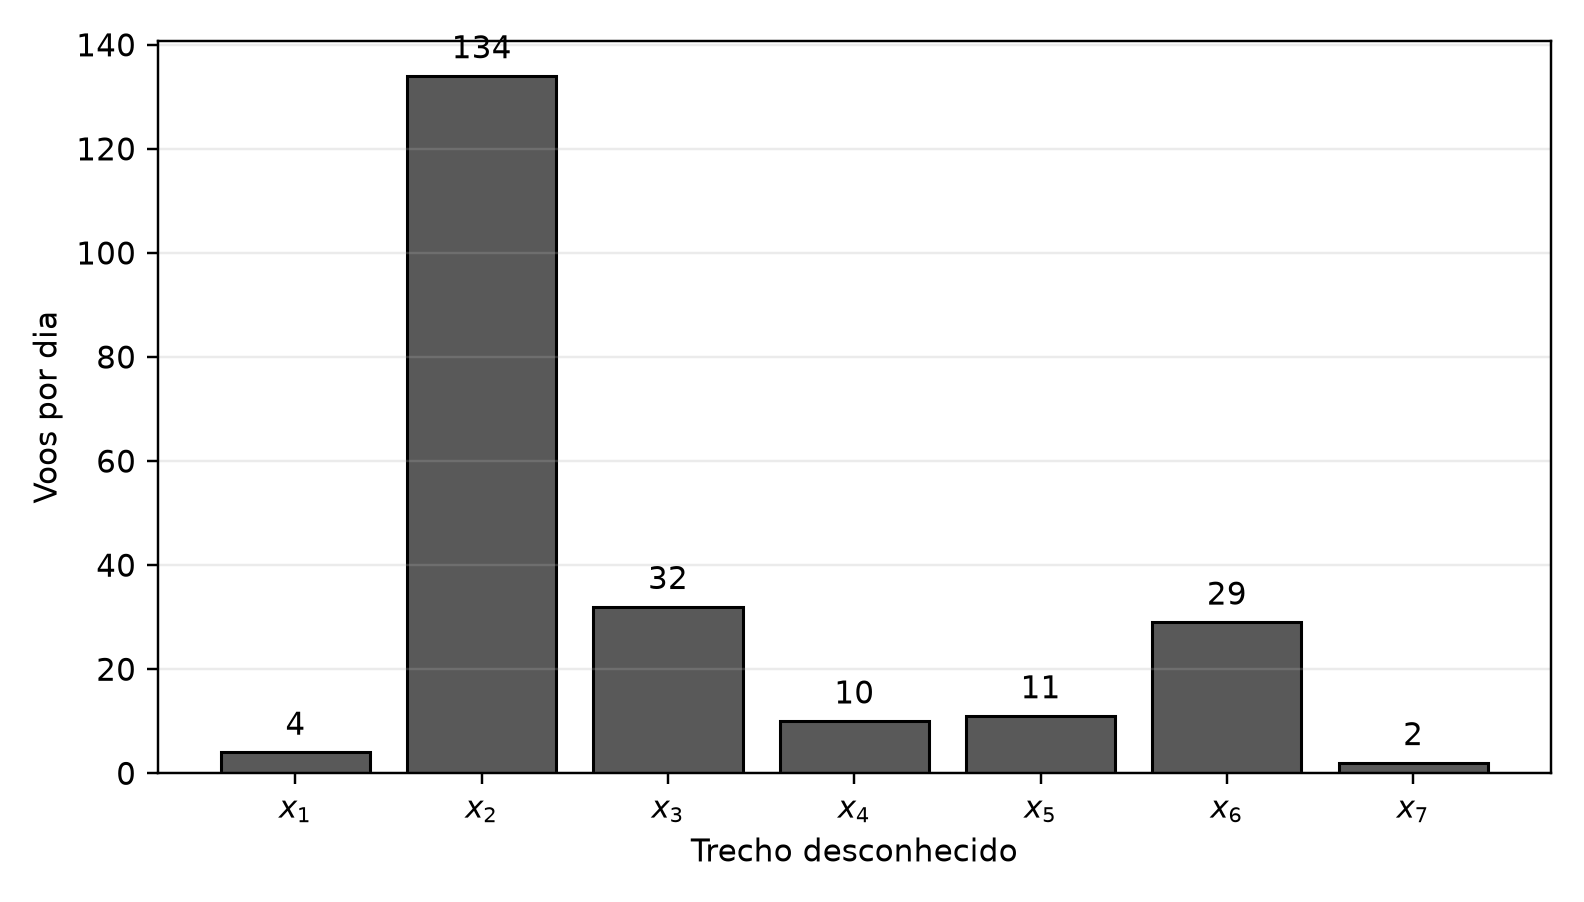
\includegraphics[width=0.78\textwidth]{figures/q2_voos_por_dia.png}
\caption{Fluxos desconhecidos obtidos para a malha aérea.}
\label{fig:q2bar}
\end{figure}

A substituição independente resultou em $Ax-b=(0,0,0,0,0,0,0)^T$ e $\lVert Ax-b\rVert_2=0$ na aritmética de ponto flutuante usada. A relação adicional também é satisfeita: $x_1=4=2\times2=2x_7$. Como diagnóstico, $\kappa_2(A)=25,433$, valor moderado para esta matriz; ele não sugere sensibilidade extrema dos fluxos a pequenas perturbações dos dados.

\subsection{Conclusão da questão}

O sistema é consistente e a solução encontrada satisfaz simultaneamente todas as equações de conservação e a relação adicional. O residual nulo confirma a substituição numérica. Embora as três primeiras etapas não tenham exigido permuta por causa de empates de magnitude, o pivotamento continua sendo parte necessária do algoritmo: em outra ordenação ou em um sistema com pivôs pequenos, ele reduz o risco de uma divisão numericamente insegura.

\section{Questão 3 -- Sistema de equações não lineares}

\subsection{Formulação e implementação}

O vetor de incógnitas foi mantido na ordem $x=[\Delta p, T_{in}, T_{out}, \mu_{med}]^T$. Para cada chute, Newton-Raphson resolve a cada passo
\begin{equation}
J(x_k)\Delta x_k=-F(x_k),\qquad x_{k+1}=x_k+\Delta x_k,
\end{equation}
por eliminação de Gauss com pivotamento parcial. A inversa de $J$ não foi formada explicitamente. A Jacobiana analítica empregada foi
\[
J(x)=\begin{bmatrix}
10^6 & 0 & 0 & -32Lv/D^2\\
0 & \dot m C_p-UA_s/2 & -\dot m C_p-UA_s/2 & 0\\
-\frac{10^6\dot m}{\eta\rho}\frac{C_{elet}24}{1000} & -\frac{\dot mC_pC_{calor}24}{1000} & 0 & 0\\
0 & 55e^{-0,1(T_{in}+T_{out})/2} & 55e^{-0,1(T_{in}+T_{out})/2} & 1
\end{bmatrix}.
\]

Os riscos teóricos examinados foram Jacobiana singular, crescimento do resíduo, iterados não finitos e sensibilização pelo chute inicial. Não foi introduzido amortecimento, retrocesso ou troca de método. Os dois casos convergiram antes do limite de 100 passos.

\subsection{Resultados}

\begin{figure}[H]
\centering
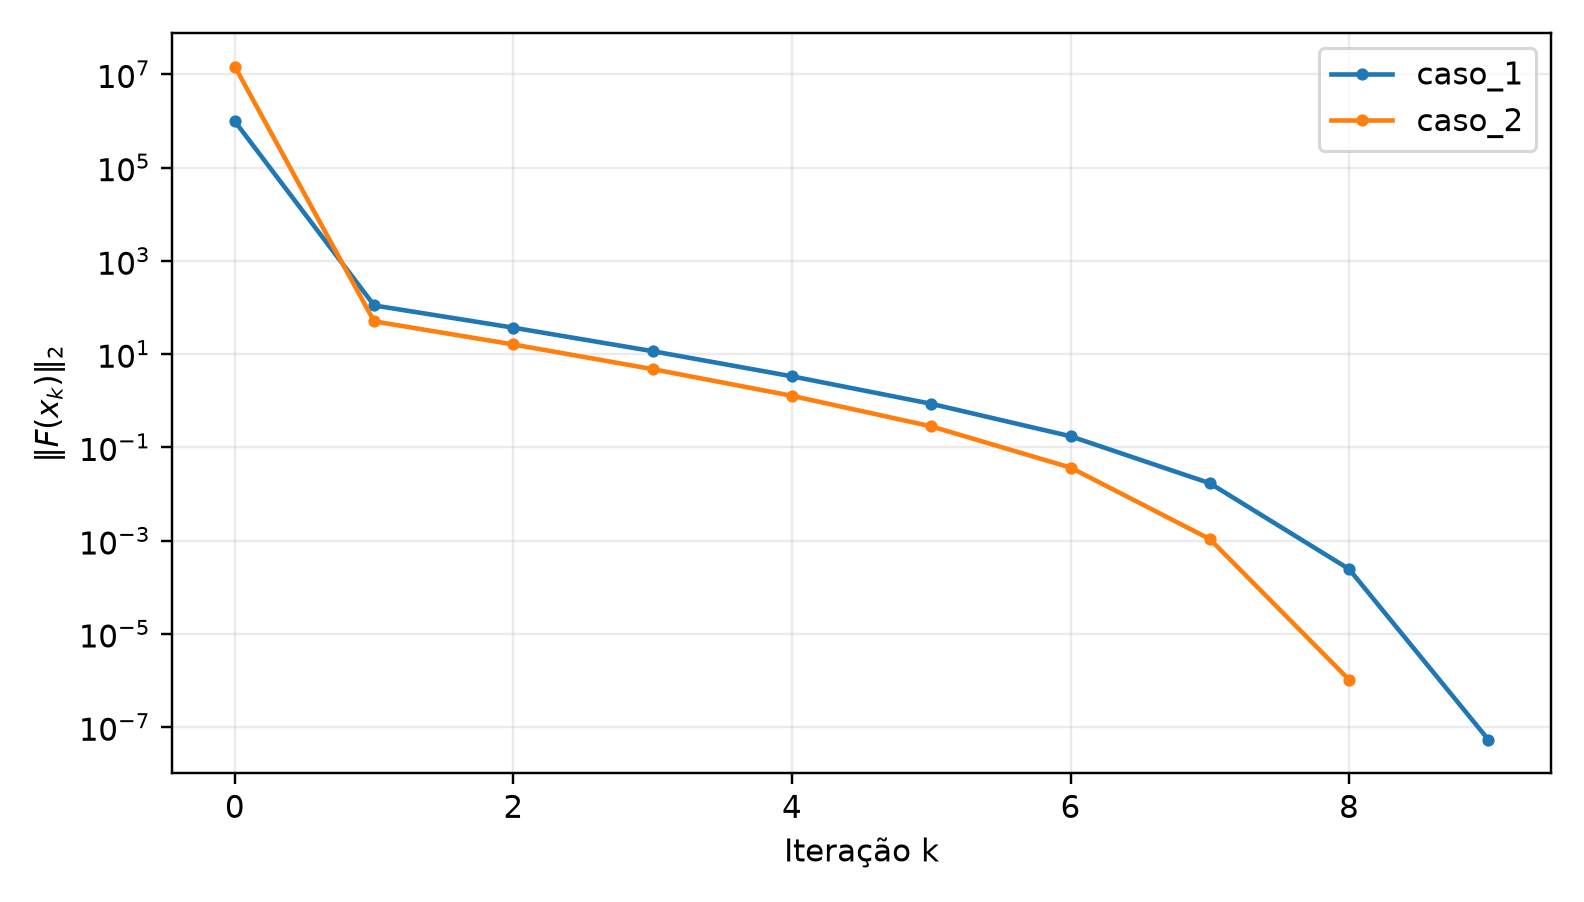
\includegraphics[width=0.79\textwidth]{figures/q3_residuo_iteracoes.png}
\caption{Norma do resíduo ao longo das iterações de Newton-Raphson.}
\label{fig:q3residuo}
\end{figure}

\begin{figure}[H]
\centering
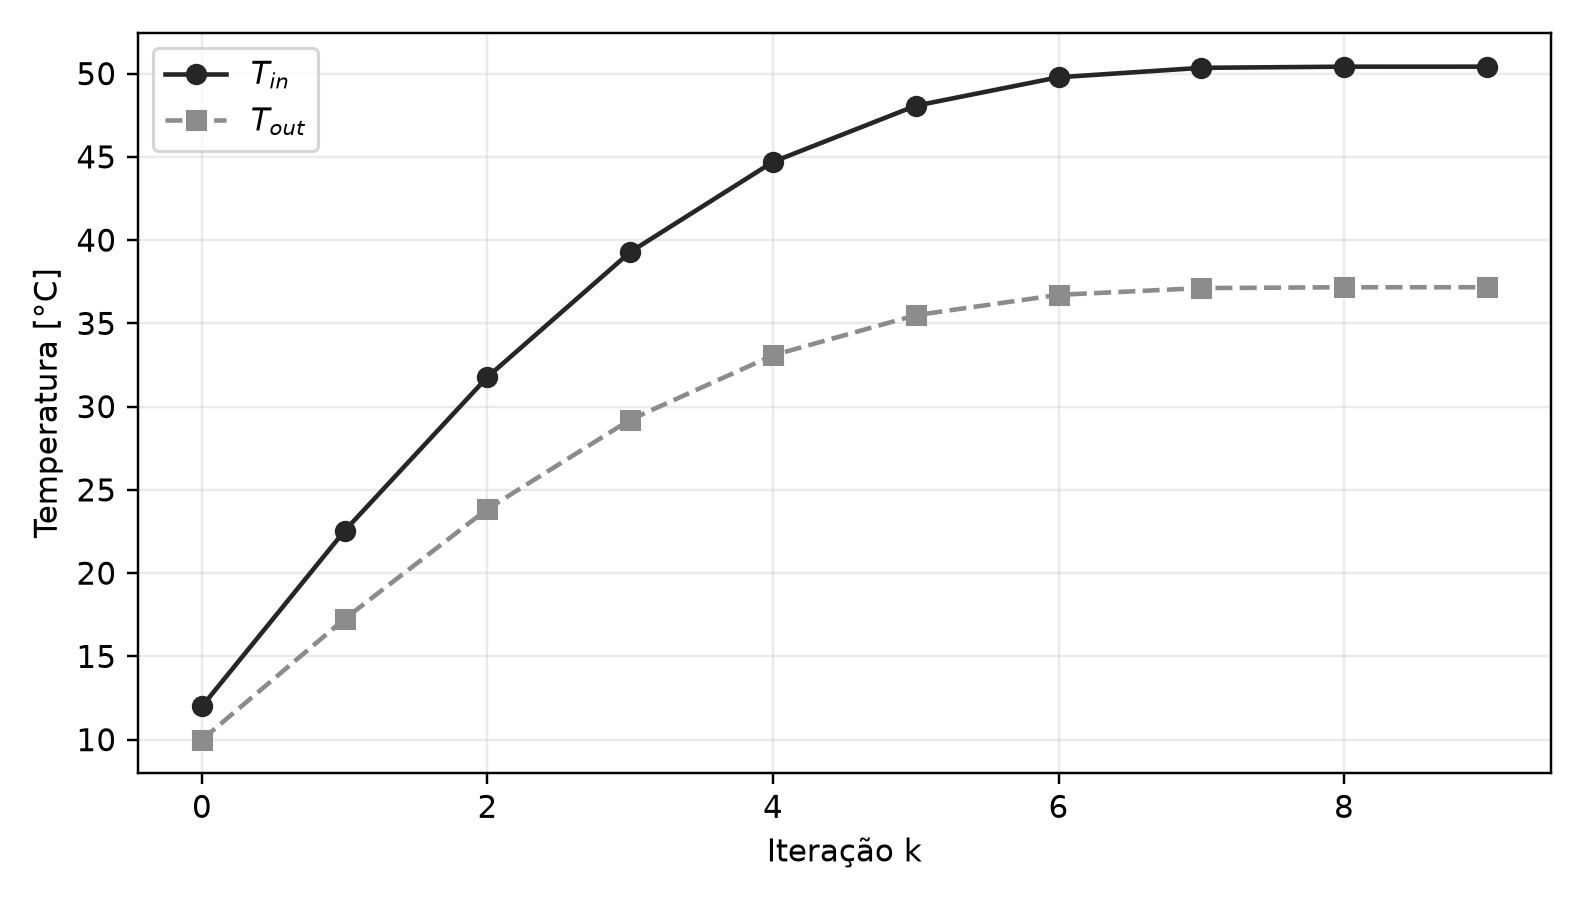
\includegraphics[width=0.78\textwidth]{figures/q3_caso_1_temperaturas.png}
\caption{Trajetória das temperaturas para o Caso 1.}
\label{fig:q3temp1}
\end{figure}

\begin{figure}[H]
\centering
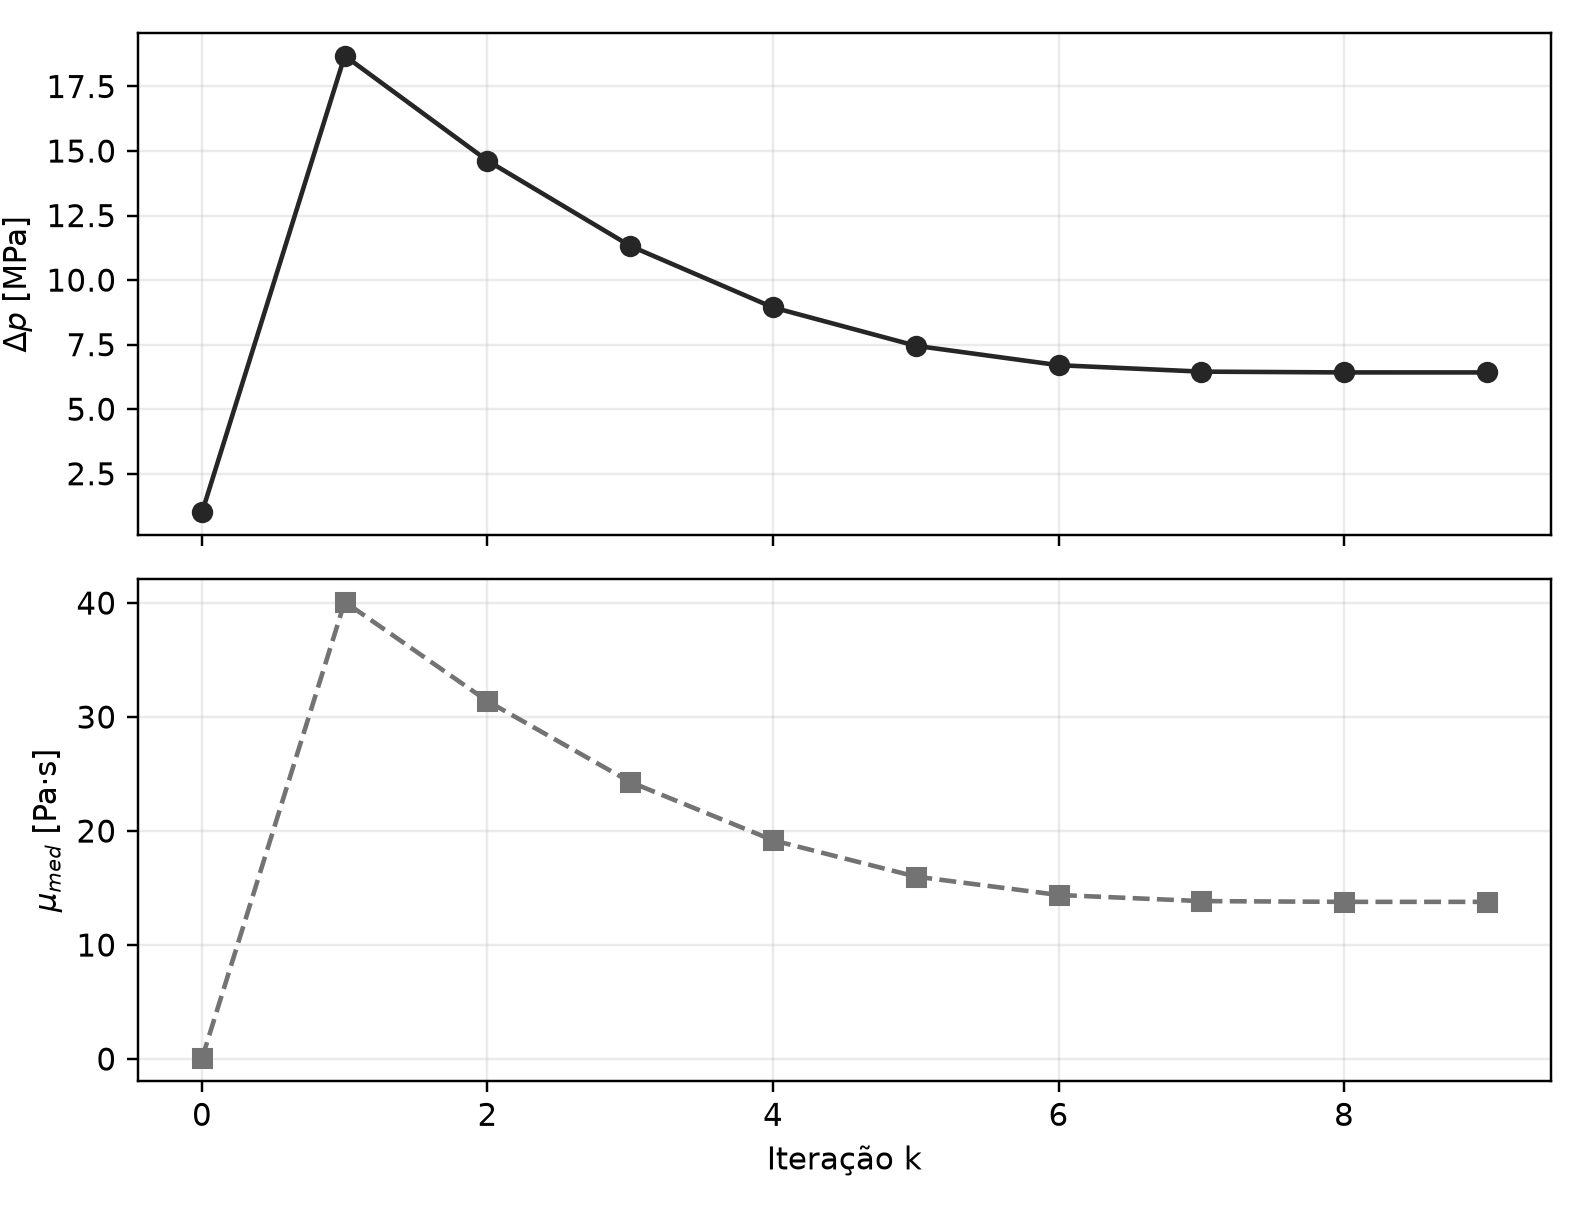
\includegraphics[width=0.78\textwidth]{figures/q3_caso_1_pressao_viscosidade.png}
\caption{Trajetória de $\Delta p$ e $\mu_{med}$ para o Caso 1.}
\label{fig:q3pv1}
\end{figure}

\begin{figure}[H]
\centering
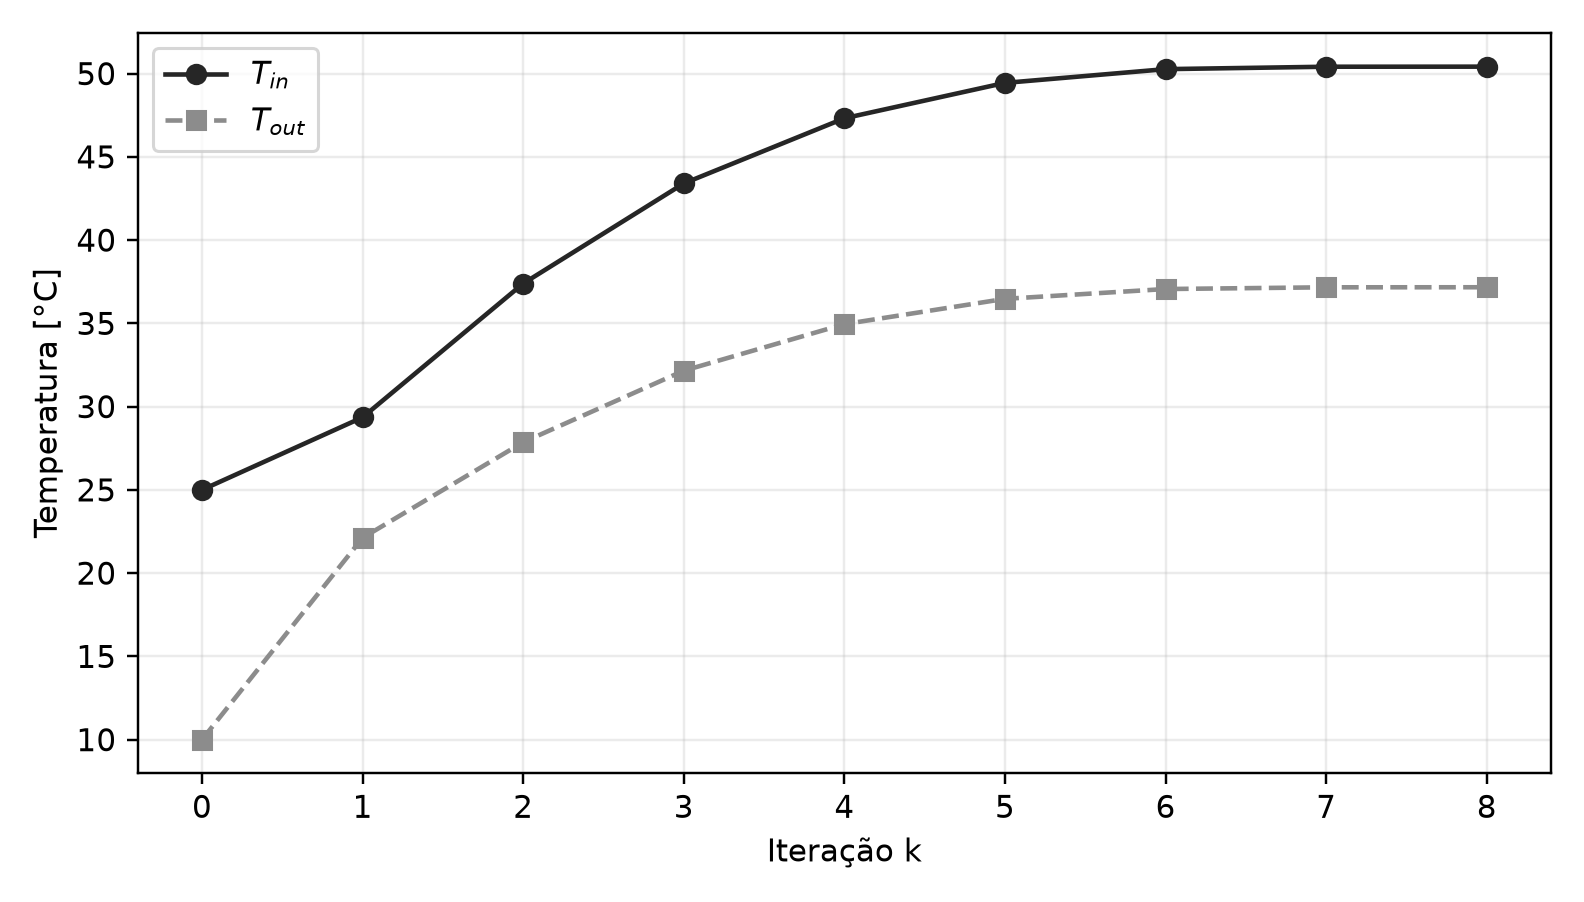
\includegraphics[width=0.78\textwidth]{figures/q3_caso_2_temperaturas.png}
\caption{Trajetória das temperaturas para o Caso 2.}
\label{fig:q3temp2}
\end{figure}

\begin{figure}[H]
\centering
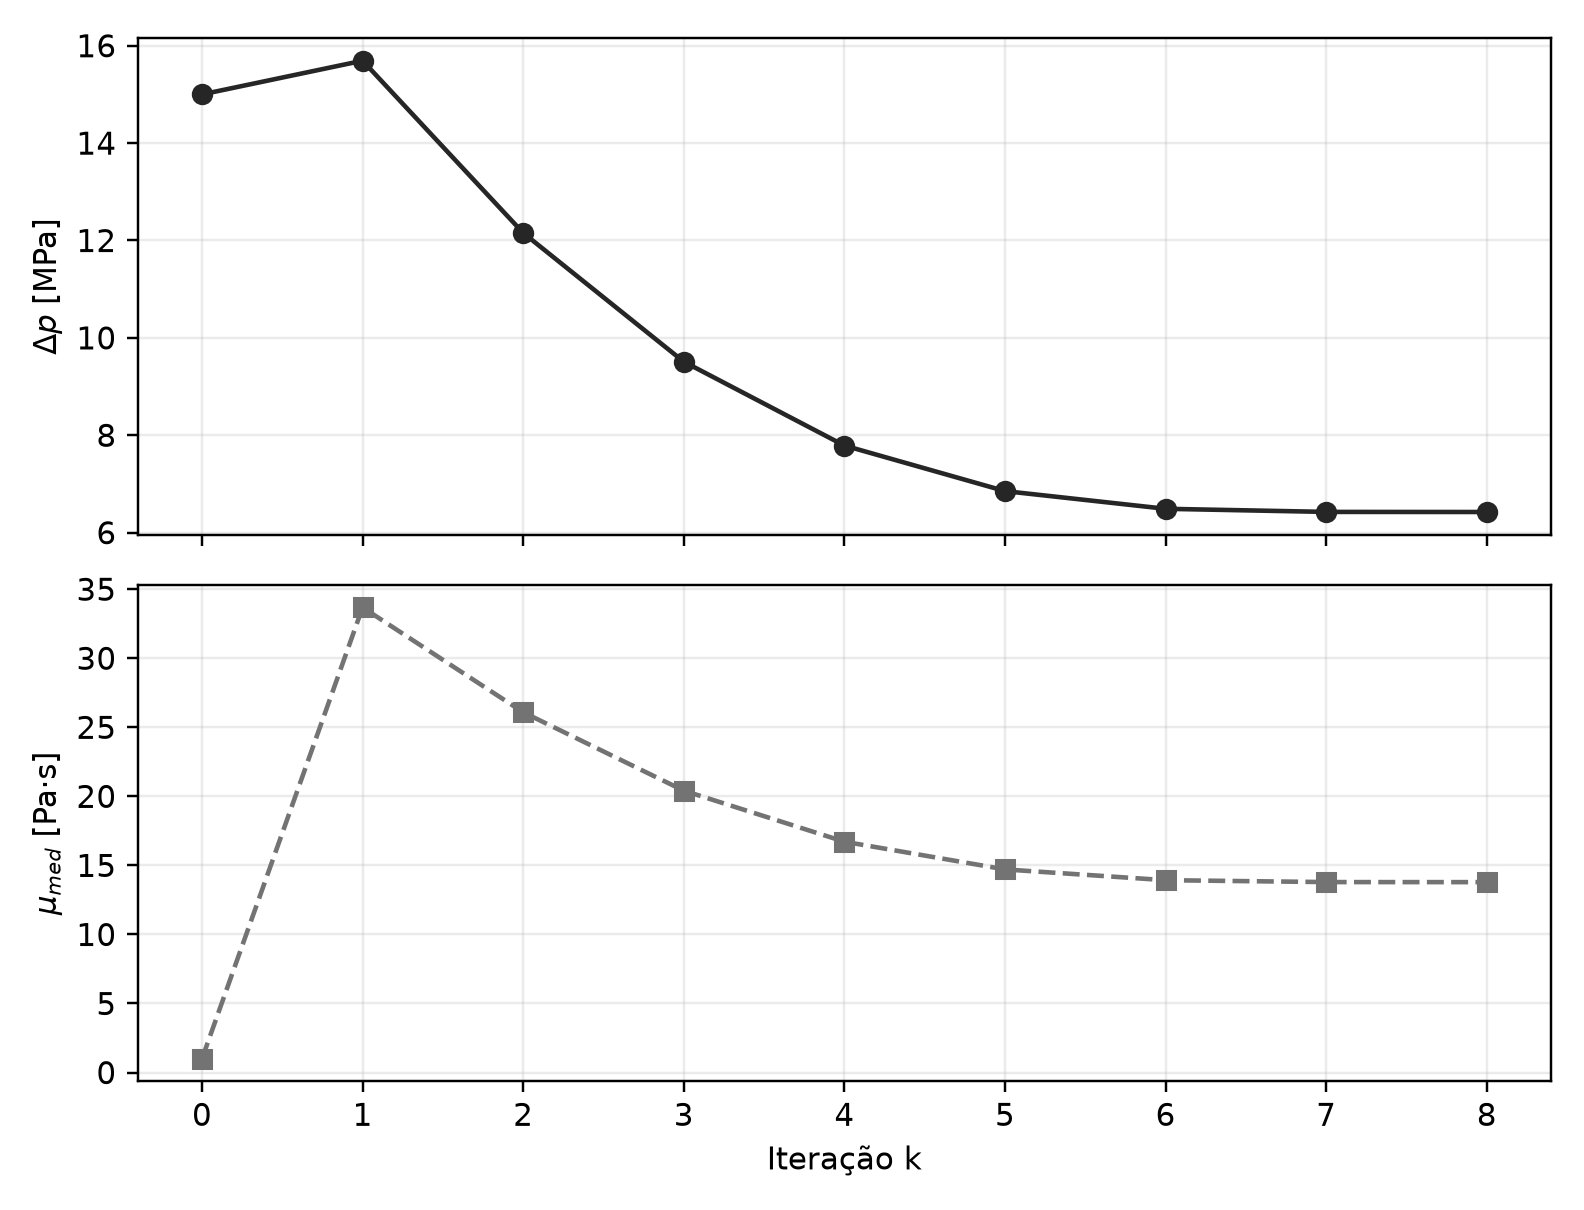
\includegraphics[width=0.78\textwidth]{figures/q3_caso_2_pressao_viscosidade.png}
\caption{Trajetória de $\Delta p$ e $\mu_{med}$ para o Caso 2.}
\label{fig:q3pv2}
\end{figure}

\begin{table}[H]
\centering
\caption{Resultado de Newton-Raphson para os dois chutes prescritos.}
\label{tab:q3}
\begin{tabular}{lrrrrrl}
\toprule
Chute & $\Delta p$ [MPa] & $T_{in}$ [°C] & $T_{out}$ [°C] & $\mu_{med}$ [Pa$\cdot$s] & Iterações & Situação \\
\midrule
Caso 1 & 6,423854 & 50,417201 & 37,168916 & 13,787461 & 9 & Convergiu \\
Caso 2 & 6,423856 & 50,417197 & 37,168913 & 13,787465 & 8 & Convergiu \\
\bottomrule
\end{tabular}
\end{table}

No Caso 1, a norma inicial foi $9,772\times10^5$ e decresceu para $5,372\times10^{-8}$ em nove atualizações. No Caso 2, a norma inicial foi $1,457\times10^7$ e atingiu $1,038\times10^{-6}$ em oito atualizações. A substituição final no vetor de equações deu, respectivamente,
\[
F(x_{\text{Caso 1}})=(-9,313\times10^{-10},0,0,-5,371\times10^{-8})^T
\]
e
\[
F(x_{\text{Caso 2}})=(9,313\times10^{-10},2,328\times10^{-10},9,095\times10^{-13},-1,038\times10^{-6})^T.
\]
Portanto, ambas as normas atendem à tolerância. O número de condição 2 da Jacobiana no final ficou próximo de $7,49\times10^6$. Esse diagnóstico é elevado porque as quatro coordenadas e as quatro equações têm escalas físicas muito diferentes; ele não substituiu o critério de parada. Nesta execução, os resíduos continuaram decrescendo e nenhuma Jacobiana singular, oscilação ou iterado não finito foi observado.

\subsection{Análise física e conclusão da questão}

Os dois chutes convergiram para a mesma solução dentro da tolerância. Em ambos, $T_{in}\approx50,42$ °C é maior que $T_{out}\approx37,17$ °C, coerente com a perda térmica do óleo ao longo do duto para o ambiente a 4 °C. A relação exponencial de viscosidade retorna $\mu_{med}\approx13,79$ Pa$\cdot$s nessa faixa de temperatura; esse valor entra diretamente na equação de perda de carga e resulta em $\Delta p\approx6,424$ MPa. O balanço econômico e as três outras relações são satisfeitos conjuntamente pelos resíduos apresentados, de modo que a solução é compatível com o custo diário ótimo de US\$ 6100 estabelecido no problema.

\section{Considerações finais}

Os resultados evidenciam três comportamentos numéricos distintos. Na equação escalar, os métodos de quebra foram previsíveis por preservarem um intervalo válido, enquanto Newton e secante foram mais rápidos para os pontos iniciais fornecidos. No sistema linear, a eliminação de Gauss com pivotamento produziu uma solução com residual nulo e tornou explícitas as operações de redução. No sistema não linear, Newton-Raphson convergiu a partir dos dois chutes sem amortecimento, embora o condicionamento da Jacobiana recomende atenção à escala das variáveis em problemas semelhantes. Em todos os casos, o residual exigido pelo enunciado foi usado como critério principal de aceitação.

\begin{thebibliography}{9}
\bibitem{enunciado} COSTA, Lucas Kuhnen; CAMPONOGARA, Eduardo. \textit{Trabalho Prático 1}. DAS-5103 -- Cálculo Numérico para Controle e Automação, UFSC, setembro de 2026.
\bibitem{notas} CAMPONOGARA, Eduardo; CASTELAN NETO, Eugênio de Bona. \textit{Cálculo Numérico para Controle e Automação}. UFSC, versão preliminar, agosto de 2008.
\end{thebibliography}

\appendix
\section{Tabelas completas de iteração}
\subsection*{Questão 1}
\begin{longtable}{rrrr}
\caption{Histórico completo do método da Bisseção na Questão 1.}\label{tab:iter-q1-1} \\
\toprule
$k$ & $\theta_k$ [rad] & $f(\theta_k)$ & $|f(\theta_k)|$ \\
\midrule
\endfirsthead
\toprule
$k$ & $\theta_k$ [rad] & $f(\theta_k)$ & $|f(\theta_k)|$ \\
\midrule
\endhead
1 & 1.000000000 & 3.225711206e+02 & 3.225711206e+02 \\
2 & 0.750000000 & 2.044757687e+02 & 2.044757687e+02 \\
3 & 0.625000000 & 8.121385981e+01 & 8.121385981e+01 \\
4 & 0.562500000 & 4.527010802e+00 & 4.527010802e+00 \\
5 & 0.531250000 & -3.734803837e+01 & 3.734803837e+01 \\
6 & 0.546875000 & -1.612444881e+01 & 1.612444881e+01 \\
7 & 0.554687500 & -5.726551791e+00 & 5.726551791e+00 \\
8 & 0.558593750 & -5.816489119e-01 & 5.816489119e-01 \\
9 & 0.560546875 & 1.977221213e+00 & 1.977221213e+00 \\
10 & 0.559570312 & 6.989199879e-01 & 6.989199879e-01 \\
11 & 0.559082031 & 5.891884330e-02 & 5.891884330e-02 \\
12 & 0.558837891 & -2.612942273e-01 & 2.612942273e-01 \\
13 & 0.558959961 & -1.011699878e-01 & 1.011699878e-01 \\
14 & 0.559020996 & -2.112114591e-02 & 2.112114591e-02 \\
15 & 0.559051514 & 1.889995532e-02 & 1.889995532e-02 \\
16 & 0.559036255 & -1.110318640e-03 & 1.110318640e-03 \\
17 & 0.559043884 & 8.894887504e-03 & 8.894887504e-03 \\
18 & 0.559040070 & 3.892301723e-03 & 3.892301723e-03 \\
19 & 0.559038162 & 1.390995864e-03 & 1.390995864e-03 \\
20 & 0.559037209 & 1.403396923e-04 & 1.403396923e-04 \\
21 & 0.559036732 & -4.849892040e-04 & 4.849892040e-04 \\
22 & 0.559036970 & -1.723246883e-04 & 1.723246883e-04 \\
23 & 0.559037089 & -1.599248117e-05 & 1.599248117e-05 \\
24 & 0.559037149 & 6.217360976e-05 & 6.217360976e-05 \\
25 & 0.559037119 & 2.309056538e-05 & 2.309056538e-05 \\
26 & 0.559037104 & 3.549042390e-06 & 3.549042390e-06 \\
\bottomrule
\end{longtable}

\begin{longtable}{rrrr}
\caption{Histórico completo do método da Falsa posição na Questão 1.}\label{tab:iter-q1-2} \\
\toprule
$k$ & $\theta_k$ [rad] & $f(\theta_k)$ & $|f(\theta_k)|$ \\
\midrule
\endfirsthead
\toprule
$k$ & $\theta_k$ [rad] & $f(\theta_k)$ & $|f(\theta_k)|$ \\
\midrule
\endhead
1 & 0.975532111 & 3.186561141e+02 & 3.186561141e+02 \\
2 & 0.596821900 & 4.783179117e+01 & 4.783179117e+01 \\
3 & 0.561004728 & 2.575760481e+00 & 2.575760481e+00 \\
4 & 0.559135072 & 1.284678378e-01 & 1.284678378e-01 \\
5 & 0.559041968 & 6.382296868e-03 & 6.382296868e-03 \\
6 & 0.559037343 & 3.170112666e-04 & 3.170112666e-04 \\
7 & 0.559037114 & 1.574592488e-05 & 1.574592488e-05 \\
8 & 0.559037102 & 7.820985957e-07 & 7.820985957e-07 \\
\bottomrule
\end{longtable}

\begin{longtable}{rrrr}
\caption{Histórico completo do método da Newton na Questão 1.}\label{tab:iter-q1-3} \\
\toprule
$k$ & $\theta_k$ [rad] & $f(\theta_k)$ & $|f(\theta_k)|$ \\
\midrule
\endfirsthead
\toprule
$k$ & $\theta_k$ [rad] & $f(\theta_k)$ & $|f(\theta_k)|$ \\
\midrule
\endhead
1 & 0.444733574 & -1.647086597e+02 & 1.647086597e+02 \\
2 & 0.550057608 & -1.187127760e+01 & 1.187127760e+01 \\
3 & 0.558965694 & -9.365077551e-02 & 9.365077551e-02 \\
4 & 0.559037097 & -6.057641144e-06 & 6.057641144e-06 \\
\bottomrule
\end{longtable}

\begin{longtable}{rrrr}
\caption{Histórico completo do método da Secante na Questão 1.}\label{tab:iter-q1-4} \\
\toprule
$k$ & $\theta_k$ [rad] & $f(\theta_k)$ & $|f(\theta_k)|$ \\
\midrule
\endfirsthead
\toprule
$k$ & $\theta_k$ [rad] & $f(\theta_k)$ & $|f(\theta_k)|$ \\
\midrule
\endhead
1 & 0.504311862 & -7.525039477e+01 & 7.525039477e+01 \\
2 & 0.574451644 & 1.993084913e+01 & 1.993084913e+01 \\
3 & 0.559764450 & 9.532227847e-01 & 9.532227847e-01 \\
4 & 0.559026730 & -1.360109528e-02 & 1.360109528e-02 \\
5 & 0.559037108 & 8.971494481e-06 & 8.971494481e-06 \\
\bottomrule
\end{longtable}

\subsection*{Questão 2}
\begin{longtable}{rrrrr}
\caption{Resumo de todas as etapas de Gauss com pivotamento na Questão 2.}\label{tab:iter-q2} \\
\toprule
Etapa & Coluna & Linha de pivô & Troca & Multiplicadores não nulos \\
\midrule
\endfirsthead
\toprule
Etapa & Coluna & Linha de pivô & Troca & Multiplicadores não nulos \\
\midrule
\endhead
1 & 1 & 1 & não & -1 \\
2 & 2 & 2 & não & -1 \\
3 & 3 & 3 & não & -1 \\
4 & 4 & 4 & não & -1 \\
5 & 5 & 5 & não & -1 \\
6 & 6 & 6 & não & 1 \\
\bottomrule
\end{longtable}

\subsection*{Questão 3}
\begin{longtable}{rrrrrr}
\caption{Histórico completo do Caso 1 (convergiu) na Questão 3.}\label{tab:iter-q3-1} \\
\toprule
$k$ & $\Delta p$ [MPa] & $T_{in}$ [°C] & $T_{out}$ [°C] & $\mu_{med}$ [Pa.s] & $\lVert F(x_k)\rVert_2$ \\
\midrule
\endfirsthead
\toprule
$k$ & $\Delta p$ [MPa] & $T_{in}$ [°C] & $T_{out}$ [°C] & $\mu_{med}$ [Pa.s] & $\lVert F(x_k)\rVert_2$ \\
\midrule
\endhead
0 & 1.000000 & 12.000000 & 10.000000 & 0.050000 & 9.771976e+05 \\
1 & 18.686490 & 22.552229 & 17.257097 & 40.106650 & 1.101882e+02 \\
2 & 14.625316 & 31.780630 & 23.851550 & 31.390187 & 3.674246e+01 \\
3 & 11.323033 & 39.284564 & 29.213730 & 24.302526 & 1.150474e+01 \\
4 & 8.940701 & 44.698051 & 33.082112 & 19.189347 & 3.322851e+00 \\
5 & 7.456774 & 48.070049 & 35.491682 & 16.004408 & 8.561815e-01 \\
6 & 6.704588 & 49.779275 & 36.713066 & 14.389999 & 1.724819e-01 \\
7 & 6.454822 & 50.346831 & 37.118631 & 13.853927 & 1.696152e-02 \\
8 & 6.424307 & 50.416172 & 37.168181 & 13.788434 & 2.445911e-04 \\
9 & 6.423854 & 50.417201 & 37.168916 & 13.787461 & 5.371766e-08 \\
\bottomrule
\end{longtable}

\begin{longtable}{rrrrrr}
\caption{Histórico completo do Caso 2 (convergiu) na Questão 3.}\label{tab:iter-q3-2} \\
\toprule
$k$ & $\Delta p$ [MPa] & $T_{in}$ [°C] & $T_{out}$ [°C] & $\mu_{med}$ [Pa.s] & $\lVert F(x_k)\rVert_2$ \\
\midrule
\endfirsthead
\toprule
$k$ & $\Delta p$ [MPa] & $T_{in}$ [°C] & $T_{out}$ [°C] & $\mu_{med}$ [Pa.s] & $\lVert F(x_k)\rVert_2$ \\
\midrule
\endhead
0 & 15.000000 & 25.000000 & 10.000000 & 1.000000 & 1.456646e+07 \\
1 & 15.692030 & 29.356684 & 22.119441 & 33.679666 & 5.018960e+01 \\
2 & 12.155553 & 37.392790 & 27.861901 & 26.089356 & 1.602257e+01 \\
3 & 9.510421 & 43.403449 & 32.157012 & 20.412132 & 4.742508e+00 \\
4 & 7.788372 & 47.316541 & 34.953239 & 16.716115 & 1.269575e+00 \\
5 & 6.853098 & 49.441810 & 36.471919 & 14.708744 & 2.811920e-01 \\
6 & 6.489727 & 50.267514 & 37.061952 & 13.928845 & 3.668498e-02 \\
7 & 6.425848 & 50.412671 & 37.165679 & 13.791740 & 1.076860e-03 \\
8 & 6.423856 & 50.417197 & 37.168913 & 13.787465 & 1.038196e-06 \\
\bottomrule
\end{longtable}

\section{Código da Questão 1}
\lstinputlisting[language=Python]{codigo_q1.py}
\section{Código da Questão 2}
\lstinputlisting[language=Python]{codigo_q2.py}
\section{Código da Questão 3}
\lstinputlisting[language=Python]{codigo_q3.py}

\end{document}
